\section{Evaluation}
\label{sec:eva}

The evaluation of our approach consists of two parts. In the first, we
evalute the benefit of using the dynamic programming query
optimization algorithm for Linked Data query processing in a
single-objective scenario. In the second part, we focus on the
multi-objective optimization approach proposed in this paper.

\subsection{Single-objective Optimization with Dynamic Programming}

\subsubsection{Systems}


\subsubsection{Results}



\begin{figure}[htb]
  \centering
  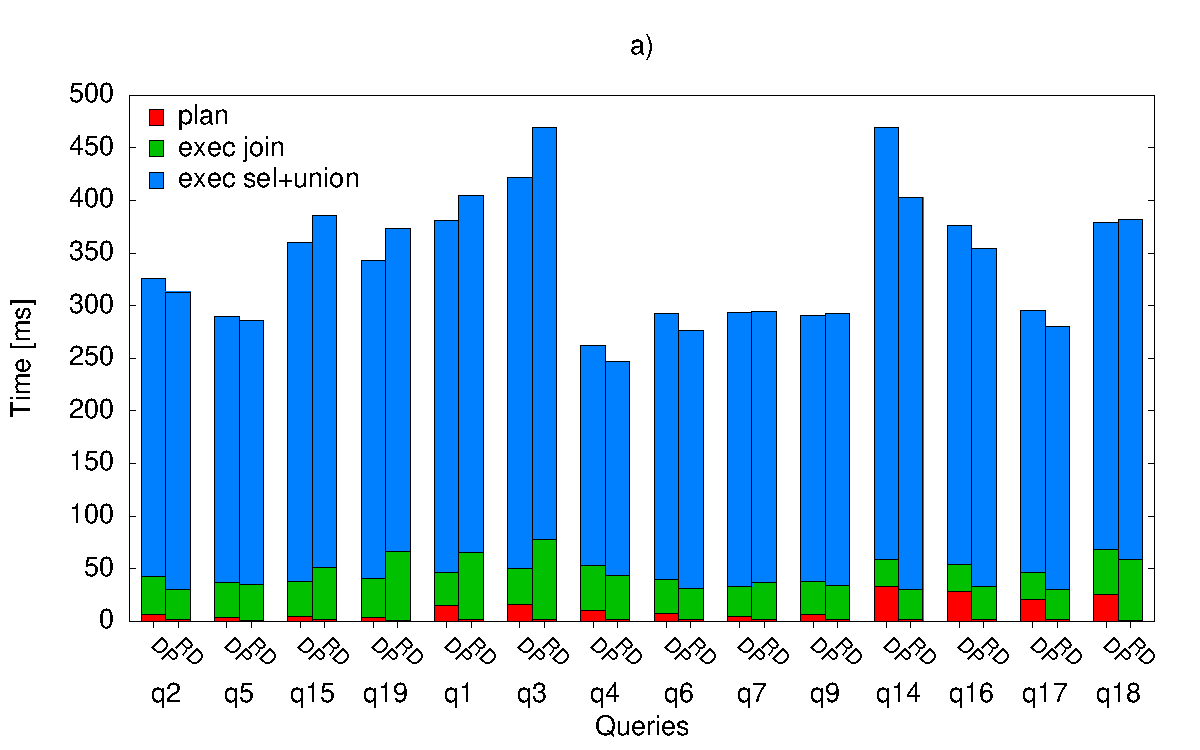
\includegraphics[width=\linewidth]{figs/exec_queries.pdf}
  \caption{Results for execution}
  \label{fig:exec_queries}
\end{figure}


\subsection{Multi-objective Optimization with Dynamic Programming}

\subsubsection{Systems}

\textbf{Baselines.} As there are no comparable source selection and
query optimization approaches that produce a range of query plans
instead of a single one, we implemented two straightforward baselines
in order to evaluate the quality of the plans produced by our new
approach. 

The first baseline (RD) is based on randomly selecting subsets of $D$
with sizes $\{1\ldots |D|\}$ (i.e., there are $|D|$ such subsets). For
each of these subsets, we create a single query plan using a standard
dynamic programming optimizer. Source scan operators are shared
between triple patterns where appropriate.

The second baseline (RK) is simliar to the first one, except that the
sources in $D$ are first ranked by the number of contained triples
that match query triple patterns (as obtained from the source index),
calculated as $score(d) = \sum_{t \in q} card_t(d)$. Instead of a
random selection, we now create subsets of $D$ by starting with the
highest ranked source and then successively adding sources in order of
their ranking to obtain $|D|$ subsets in total. For each subset, we
build a query plan in the same manner as for baseline RD.

\todo{explain modifications to create more plans}

\textbf{Our Approach.} We implemented two versions of our
approach. The first version (DP) obtains the complete set of
Pareto-optimal plans as described in the previous sections. The second
version (DPU) does not use bounds as described in
Section~\ref{sec:sharing} (i.e., while operator sharing is employed,
its effect are not taken into account during pruning) and therefore
will not compute the correct Pareto-optimal set of plans. However,
pruning is more effective and should lead to faster performance.

\textbf{Parameters.} Parameter $b$ specifies the benefit that is
assumed during query planning for sharing of source scan
operators. For example, with $b=0.8$ the planners assume that 80\% of
the source scan cost is saved, i.e., second and subsequent reads of a
source scan operator cost only 20\% of the first read.

For RD and RK, parameter $m$ describes the number of additional plans
that were generated by randomly removing source scan operators.

\subsubsection{Datasets and Queries}

We created 14 BGP queries of different sizes w.r.t. to the number of
triple patterns. We executed all queries using a link traversal
approach and recorded all retrieved sources. This dataset was then
indexed in a source index and used for the evaluation. The dataset
consists of 1,909,109 triples and contains data from various popular
open datasets, such as DBpedia, Freebase, New York Times, GeoNames,
LinkedMDB and others. 

\todo{describe how sources were aggregated to host-sources}

Table~\ref{tab:queries} shows various statistics for all evaluation
queries.

\begin{table}[htb]
  \centering
  \begin{tabular}{l|c|c|r|r|r|r}
    Query & \#Pat. & \#Src. & \#Src./Pat. (SD) & Shared [kT] & \#Res. & Join-Sel. SD \\ 
    \hline

    Q2  & 3 & 13 & 5.33 (6.66) & 1,175 & 24  & 2.36\textsc{e}-5 \\
    Q5  & 3 & 13 & 5.00 (6.93) & 633   & 13  & 5.73\textsc{e}-5 \\
    Q15 & 3 & 13 & 5.33 (6.66) & 1,245 & 11  & 3.95\textsc{e}-5 \\
    Q19 & 3 & 13 & 7.33 (6.03) & 1,329 & 918 & 4.36\textsc{e}-5 \\
    \hline
    Q1  & 4 & 13 & 4.75 (5.56) & 1,296 & 2   & 1.30\textsc{e}-3 \\
    Q3  & 4 & 13 & 4.75 (5.56) & 1,762 & 3   & 1.89\textsc{e}-5 \\
    Q4  & 4 & 13 & 4.00 (6.00) & 50    & 60  & 9.58\textsc{e}-3 \\
    Q6  & 4 & 13 & 4.00 (6.00) & 594   & 6   & 2.62\textsc{e}-3 \\
    Q7  & 4 & 13 & 4.75 (5.68) & 702   & 106 & 2.75\textsc{e}-3 \\
    \hline
    Q9  & 5 & 13 & 4.60 (5.37) & 703   & 17  & 5.26\textsc{e}-3 \\
    Q14 & 5 & 8  & 2.60 (3.05) & 1729  & 20  & 3.71\textsc{e}-3 \\
    Q16 & 5 & 13 & 3.80 (5.22) & 951   & 1   & 2.10\textsc{e}-3 \\
    Q17 & 5 & 13 & 3.40 (5.37) & 599   & 1   & 8.92\textsc{e}-3 \\
    Q18 & 5 & 10 & 3.00 (3.39) & 970   & 2   & 1.21\textsc{e}-4 \\
  \end{tabular}
  \caption{Query statistics: query name, number of patterns, number of unique sources, average number of sources per pattern (standard deviation), number of triples (in thousands) contained in shared sources, number results, standard deviation of selectivies of all joins in query.}
  \label{tab:queries}
\end{table}

\begin{table}[htb]
  \centering
  \begin{tabular}{l|r|r|r|r|r|r|r|r|r|r|r|r|r|r|r|r}
 & RD & RK & DP & DPU & RD & RK & DP & DPU & RD & RK & DP & DPU & RD & RK & DP & DPU \\
    \hline               
                                                                                                               
 & \multicolumn{4}{c}{Q2} & \multicolumn{4}{|c|}{Q5} & \multicolumn{4}{c}{Q15} & \multicolumn{4}{|c}{Q19}  \\

    \hline                                                                                                   

    \#Plans   & 1702 & 1853 & 673   & 619  & 1382 & 1871 & 446   & 446   & 2376 & 3263 & 634   & 634   & 3817 & 3240 & 761   & 761   \\
    \#Skyline & 153  & 155  & 673   & 575  & 106  & 176  & 446   & 446   & 13   & 40   & 634   & 634   & 41   & 46   & 761   & 761   \\ 
    \%Skyline & 22.7 & 23.0 & 100.0 & 85.4 & 23.8 & 39.5 & 100.0 & 100.0 & 2.1  & 6.3  & 100.0 & 100.0 & 5.4  & 6.0  & 100.0 & 100.0 \\
    Time [s]  & 1.06 & 0.92 & 1.14  & 0.62 & 0.78 & 1.03 & 0.75  & 0.53  & 1.05 & 1.14 & 1.21  & 0.64  & 1.07 & 1.05 & 1.58  & 0.77  \\
  
    \hline
    \hline

 & \multicolumn{4}{c}{Q1} & \multicolumn{4}{|c|}{Q3} & \multicolumn{4}{c|}{Q4} & \multicolumn{4}{c}{Q6} \\

    \hline

    \#Plans   & 3945 & 5362 & 866   & 832  & 4571 & 5153 & 901   & 847  & 1471 & 1306 & 453   & 465  & 954  & 1340 & 354   & 318  \\
    \#Skyline & 0    & 0    & 866   & 689  & 0    & 0    & 901   & 699  & 1    & 0    & 453   & 434  & 0    & 1    & 354   & 283  \\ 
    \%Skyline & 0.0  & 0.0  & 100.0 & 79.6 & 0.0  & 0.0  & 100.0 & 77.6 & 0.2  & 0.0  & 100.0 & 95.8 & 0.0  & 0.2  & 100.0 & 79.9 \\
    Time [s]  & 1.53 & 1.67 & 7.64  & 1.60 & 1.53 & 1.62 & 10.05 & 1.80 & 1.61 & 1.29 & 1.37  & 0.75 & 1.14 & 1.33 & 1.35  & 0.70 \\

    \hline
    \hline

 & \multicolumn{4}{c}{Q7} & \multicolumn{4}{|c|}{Q9} & \multicolumn{4}{c|}{Q14} & \multicolumn{4}{c}{Q16} \\

    \hline

    \#Plans   & 2566 & 3913 & 1035  & 813  & 2622 & 3450 & 689   & 655  & 429  & 436  & 284   & 281  & 1485 & 2265 & 685   & 663  \\
    \#Skyline & 1    & 0    & 1035  & 781  & 0    & 0    & 689   & 637  & 0    & 0    & 284   & 281  & 0    & 0    & 685   & 583  \\ 
    \%Skyline & 0.1  & 0.0  & 100.0 & 75.5 & 0.0  & 0.0  & 100.0 & 92.5 & 0.0  & 0.0  & 100.0 & 98.9 & 0.0  & 0.0  & 100.0 & 85.1 \\
    Time [s]  & 1.91 & 1.50 & 20.88 & 2.28 & 1.80 & 1.64 & 23.64 & 2.56 & 1.33 & 1.21 & 0.91  & 0.41 & 1.82 & 1.99 & 14.31 & 2.38 \\

    \hline
    \hline

 & \multicolumn{4}{c}{Q17} & \multicolumn{4}{|c|}{Q18} & \multicolumn{8}{c}{} \\

    \hline

    \#Plans   & 837  & 1022 & 398   & 286   & 1021 & 1192 & 633   & 633   & \multicolumn{8}{c}{} \\
    \#Skyline & 1    & 0    & 398   & 286   & 0    & 0    & 633   & 633   & \multicolumn{8}{c}{} \\ 
    \%Skyline & 0.2  & 0.0  & 100.0 & 100.0 & 0.0  & 0.0  & 100.0 & 100.0 & \multicolumn{8}{c}{} \\
    Time [ms] & 1.67 & 1.70 & 2.68  & 0.66  & 1.53 & 1.58 & 4.15  & 1.35  & \multicolumn{8}{c}{} \\

  \end{tabular}
  \caption{Results for all queries, with $m=2000$ and $b=0.8$ for RD and RK.}
  \label{tab:res}
\end{table}

\subsubsection{Results}

Table~\ref{tab:res} shows an overview of all queries for all systems
with $b=0.8$ and $m=2000$. \todo{add averages here}

\textbf{Effect of Query Size.} Figs.~\ref{fig:pareto_tp}a+b show the
planning time and found skyline fraction for different query sizes
(i.e., number of triple patterns). An increased number of triple
patterns results in a larger search space for the query optimizer: for
all systems planning time increases with the number of triple
patterns. However, the DP algorithm is much more affected than DPU, RK
and RD. Going from 3 to 5 triple patterns, the planning time of DP
increases by a factor of 7.6, whereas the other systems' planning
times only increase by factors between 1.6 (RK) and 2.3 (DPU). 

Fig.~\ref{fig:pareto_tp}b shows the fractions of the complete plan
skyline (i.e., the plans computed by DP) that the systems are able to
calculate for different query sizes. 

\begin{figure}[htb]
  \centering
  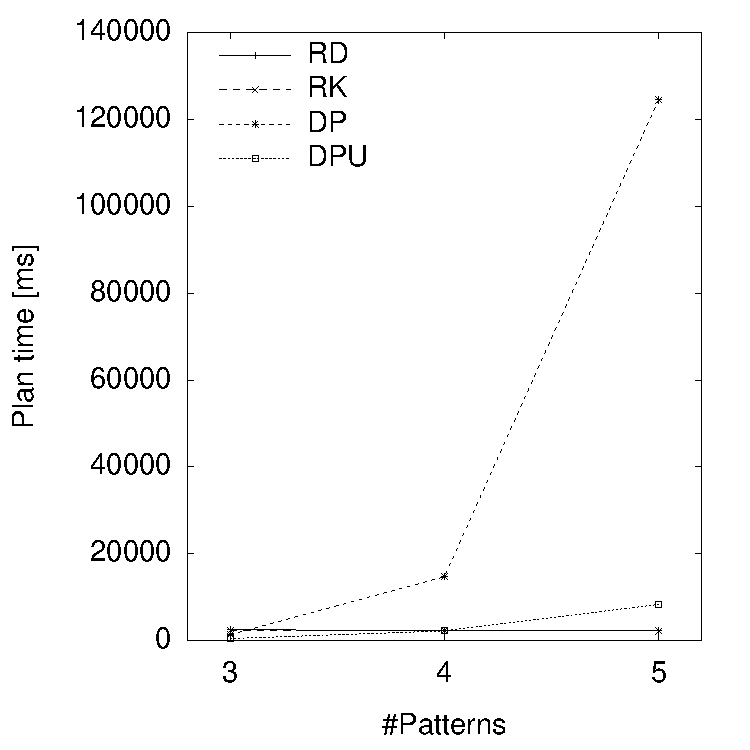
\includegraphics[width=0.49\linewidth]{figs/pareto_plan_tp.pdf}
  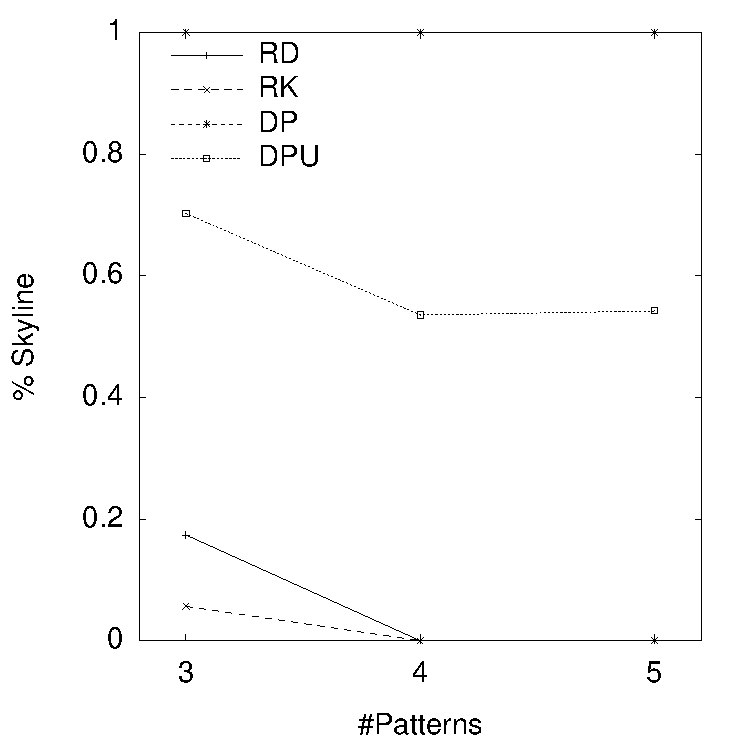
\includegraphics[width=0.49\linewidth]{figs/plans_skyline_by_tp.pdf}
  \caption{Effect of query size on a) planning time and b) skyline fractions.}
  \label{fig:pareto_tp}
\end{figure}

\textbf{Effect of Sharing Benefit.} Figs.~\ref{fig:pareto_sharing}a+b
show the planning time and skyline fractions for different values of
$b$. We see in Fig.~\ref{fig:pareto_sharing}a that the planning time
for DP increases with higher sharing benefits: from 3.3s for $b=0.1$
to 6.4s for $b=0.8$. However, the planning time for the other
approaches, DPU, RD, and RK, remain the same for all values of
$b$. The planning time for DP increases with higher sharing benefits
because the bounds of plan costs are less tight and less plans can be
pruned during the query optimization process. The other approaches are
not affected because DP is the only one that actually considers the
sharing benefit during optimization.

Fig.~\ref{fig:pareto_sharing}b shows the skyline fractions for all
approaches for different values of $b$. We can see that DPU computes a
larger part of the skyline when the sharing benefit is lower. This is
due to the fact that DPU does not take the effect of operating sharing
into account, leading to worse results the more pronounved the
influence of the sharing benefit is. The other approaches, RD and RK,
are not affected by the sharing benefit as the benefit is not taken
into account during planning.

\begin{figure}[htb]
  \centering
  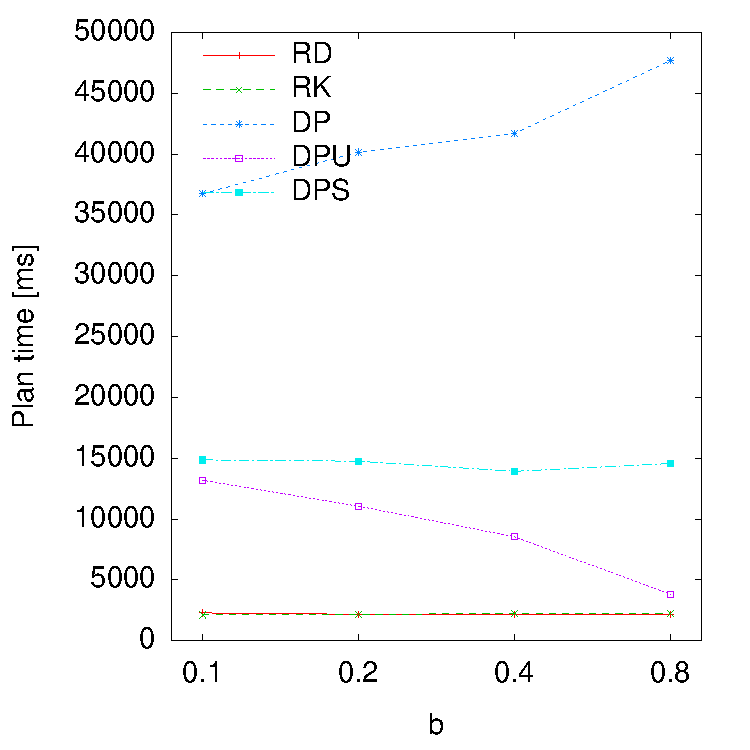
\includegraphics[width=0.49\linewidth]{figs/pareto_plan_b.pdf}
  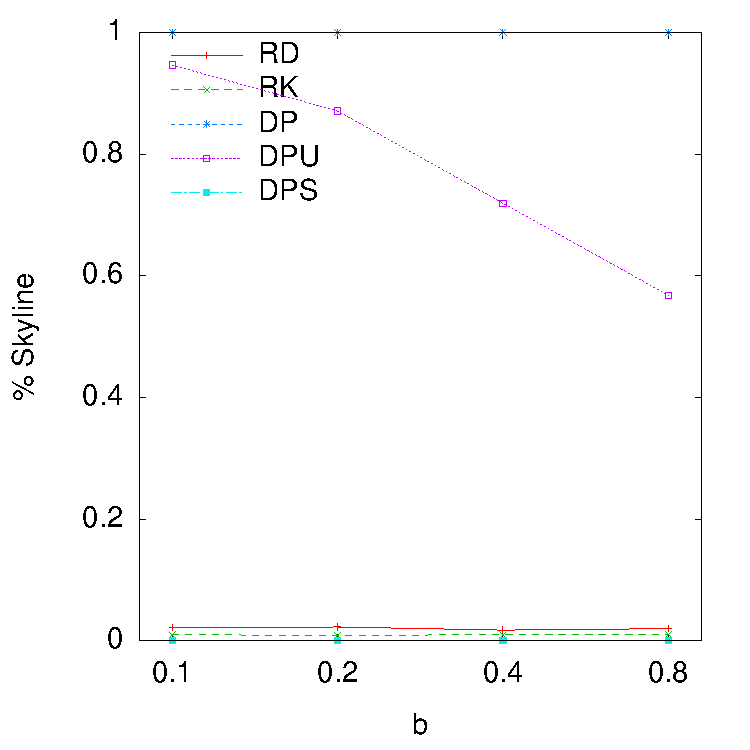
\includegraphics[width=0.49\linewidth]{figs/plans_skyline_by_b.pdf}
  \caption{Effect of sharing benefit on a) planning time and b)
    skyline fractions.}
  \label{fig:pareto_sharing}
\end{figure}

\textbf{Plan Skyline.} Figs.~\ref{fig:pareto_q2_skyline}a+b show a scatter
plot of cost and cardinality of plans generated by all systems for
query Q2. In these plots a plan dominates all plans that are to its
lower right, i.e. that have higher cost (x-axis) and lower cardinality
(y-axis). Fig.~\ref{fig:pareto_q2_skyline}a shows all plans that were
generated by the different systems. We can immediately see that many
of the plans generated by the RD and RK baselines are dominated by
other plans. Fig.~\ref{fig:pareto_q2_skyline}b shows only the plans
for all systems that are on the skyline. Here, the dominated plans in
the center of the plot no longer appear and only few RD and RK plans
remain.

\begin{figure}[htb]
  \centering
  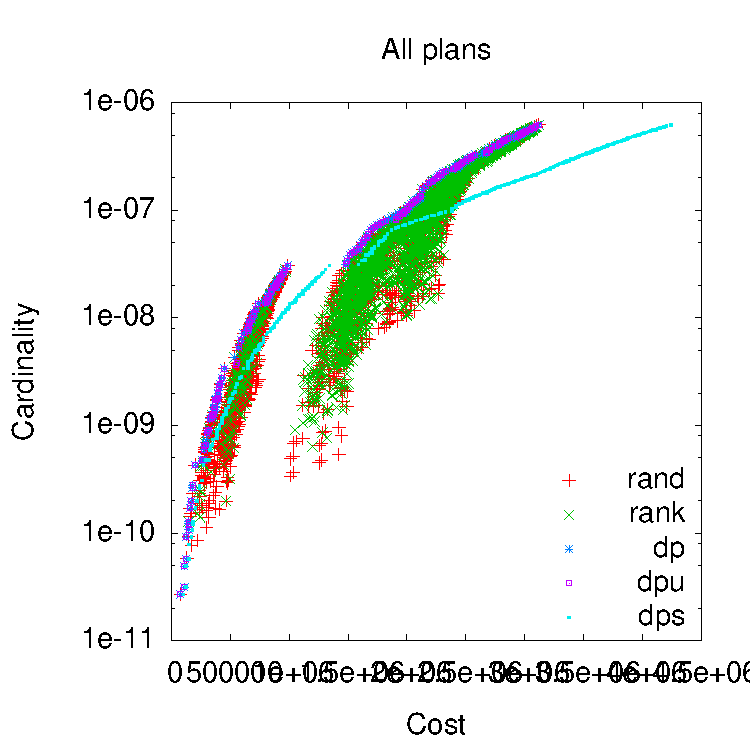
\includegraphics[width=0.49\linewidth]{figs/plans_q2_all.pdf}
  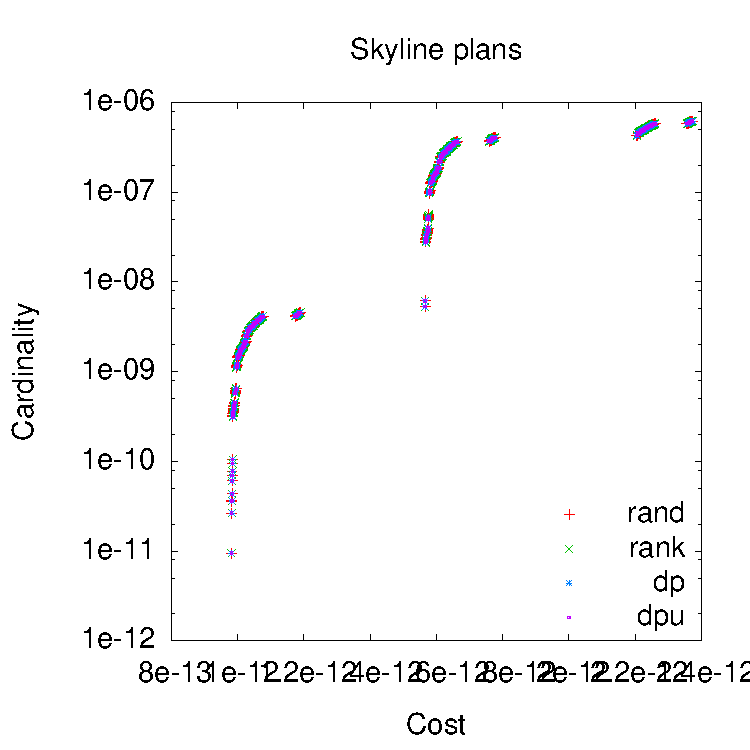
\includegraphics[width=0.49\linewidth]{figs/plans_q2_sky.pdf}
  \caption{Plans for query Q2 on all systems: a) all plans and b)
    skyline plans.}
  \label{fig:pareto_q2_skyline}
\end{figure}

\textbf{Execution Time.} \todo{execute several plans of some
  queries and show that execution time is better with fewer sources}

%%% Local Variables: 
%%% mode: latex
%%% TeX-master: "paper"
%%% End: 
